\section{Simulation setup}
\label{section:sim_setup}

Critical parameters in this system include fluid density $\rho_f$, dynamic viscosity $\eta$, surface tension $\sigma$, 
length scale $L$, and applied magnetic field strength $B$. The dynamic viscosity and surface tension is determined 
by the relaxation time using the BGK collision operator, $\eta = \rho_f c_s^2(\tau - \frac{1}{2})$ and $g_{kk'}$ 
respectively. Dimensionless numbers derived from the Buckingham Pi theorem are the Reynolds number
($Re = \frac{\rho u L}{\eta}$), Weber number ($We = \frac{\rho u^2 L}{\sigma}$), and magnetic bond number 
($\Bar{B} = \frac{Bd}{\sigma A}$). Here, $u$ is velocity, $d$ is the particle's dipole moment, and $A$ is the 
particle's cross-sectional area. The system's velocity and length scale are set as the domain size and coarsening rate. 
Parameters for the fluid, particle, and non-ideal mixing model used in the simulations are summarized in Table 
\ref{table:model_params}.

% \begin{table}[h!]
% \centering
% \begin{tabular}{||c c c c c c c c c c c c c||} 
%  \hline
%  $t_{sim}$ & $L_x$ & $\rho_f$ & $\tau$ & $\eta_f$ & $g_{cc'}$ & $\sigma$ & $\phi_f$ & $\rho_p$ & $\phi_p$ & $V_p$ & $d_c$ & $K_H$ \\ [0.5ex] 
%  \hline\hline
%  $10^5$ & 256 & 0.7 & 1 & 0.117 & 0.08 & 0.0267 & 0.5 & 1 & 0.15 & 2000$\pi$ & 2/3 & 100\\ [1ex] 
%  \hline
% \end{tabular}
% \caption{Summary of the fluid, particle and model parameters used in the proposed simulations}
% \label{table:model_params}
% \end{table}

\begin{table}
    \centering
    \caption{Summary of the parameters corresponding to the fluid, particle and model used in the simulations}
    \label{table:model_params}
    \begin{tabular}{|c|r|}
    \hline
    % Parameter & Value \\
    % \hline
    $L_V/\Delta x$ & 256 \\
    $\rho \cdot (\Delta x)^3/\Delta m$ & 0.7 \\
    $\nu \cdot \Delta t/(\Delta x)^2$ & 1/6 \\
    $\sigma \cdot (\Delta t)^2/\Delta m$ & 0.0267 \\
    $\tau/\Delta t$ & 1 \\
    $g \cdot \Delta m(\Delta t)^2/(\Delta x)^5$ & 0.08 \\
    $\phi_f$ & 0.5 \\
    $\phi_p$ & 0.15 \\
    $n_p$ & 1200 \\
    $\rho_p \cdot (\Delta x)^3/\Delta m$ & 1 \\
    $V_p/(\Delta x)^3$ & $2000\pi/3$ \\
    $m/(\Delta i(\Delta x)^2)$ & 1 \\
    $d_c/\Delta x$ & 2/3 \\
    $K_H\cdot (\Delta x)^{1/2}(\Delta t)^2/\Delta m$ & 100 \\
    \hline
    \end{tabular}
\end{table}

In these simulations, the aspect ratio is defined as $\alpha = \frac{R_{\parallel}}{R_{\perp}}$ with $\alpha = 0.5, 1, 2$ 
used in these simulations. All particle geometries are volume matched, based on the spherical particle volume. For the 
spherical particle, the radius was set at $R_{\parallel} = R_{\perp} = 7.9 \Delta x$ which sets the $\alpha = 0.5$ particles to 
$R_{\parallel} = 5 \Delta x, R_{\perp} = 10 \Delta x$ and the $\alpha = 2$ particles to $R_{\parallel} = 12.6, R_{\perp} = 6.3 \Delta x$. 
$R_{\parallel}$ and $R_{\perp}$ is the radius of the particle parallel and perpendicular to the symmetry axis of 
the particle respectively. These values are identical to what was used in Gunther et al, allowing comparisons to the 
trends they observed. \cite{gunther_timescales_2014} The particles were randomly placed in the system and an equilibration
step was performed to push the particles further away from each after placement. Once equilibration is performed, a 
constant magnetic field is switched on with dimensionless strengths defined using $\bar{B}$.

The initial condition of the system when simulating bijels sets the density of each grid to $0.5\rho_f + \varepsilon$ of 
each fluid where $\varepsilon = 0.0001N(0,1)$. The model parameters trigger phase separation with a sharp interface at 
the start of the simulation. Periodic boundary conditions are applied on all sides unless the system is undergoing shear. 
The shear gradient is applied as a velocity in the z direction across the x axis and implemented as a Lees-Edwards 
(LE) boundary condition in the yz planes. \cite{wagner_leesedwards_2002, lorenz_lees-edwards_2009, yang_capillary_2022} 
These boundaries move with velocities $u_{LE}$ and $-u_{LE}$ to conserve momentum, with a shear rate 
$\dot{\gamma} = \frac{2 u_{LE}}{L_x}$. LE boundaries are preferred over walls to avoid affecting viscosity measurements. 
\cite{wagner_leesedwards_2002, lorenz_lees-edwards_2009, yang_capillary_2022}

Bijel templates have been synthesized using water/2-6-lutidine for further applications. \cite{lee_making_2013} 
While intrinsically polymerizable bijels have been prepared using oligomeric polymers, STRIPS and VIPS currently 
utilize small molecule liquids in their bijel casting mixtures. Therefore, an experimentally viable system using 
water/2-6-lutidine will be discussed in the context of the work presented here. The critical temperature (UCST) 
for this system is $T_c = 34 ^{\circ}\text{C}$, with many systems heated to $T = 40^{\circ}\text{C}$ to form the bijel. At this 
temperature, the fluid properties are $\sigma = 0.22 \text{mN/m}$ and $\eta = 2.38 \text{mPas}$. \cite{grattoni_lower_1993} 
Fei et al. developed a method to synthesize polystyrene microparticles ($(R_p = 2 \text{\mu m})$) with tunable geometries 
by mechanically stretching or compressing them, then coating them with nickel to create magnetic microparticles with 
a dipole moment of approximately$\approx 3 \cdot 10^{-14} \text{Am^2}$. \cite{fei_active_2017, fei_magneto-capillary_2020} 
Comparing the physical properties to simulation parameters, the simulations correspond to a length scale of
$\Delta x = 252 \cdot 10^{-9} \text{m}$, timescale of $\Delta t = 624 \cdot 10^{-9} \text{s}$, 
mass scale of $\Delta m = 2.24 \cdot 10^{-15} \text{kg}$ and charge scale of $\Delta q = 2.948 \cdot 10^{-7} \text{C}$. 

\section{Model results}
\label{section:model_results}

\subsection{Surface tension}
\label{section:model_surface_tension}

In experiments, Wilhelmy and ring tensionometry are used to measure the surface tension from the force needed 
to break through the interface. Pendant drop tensionometry is also used by measuring the pressure required to 
maintain a droplet of analyte at a various sizes and utilizing the Young-Laplace equation to calculate the 
surface tension of the system. \cite{sun_assembly_2013, berry_measurement_2015}
Upon extrusion of a droplet from a reservoir, the size of a droplet is determined by the balance between 
cohesive forces between bubble molecules and geometrical forces that attempt to reduce the curvature of a 
system by increasing its size. For spherical droplets, the equation simplifies to 
$\Delta P = \frac{2 \sigma}{R_d}$ where $\Delta P$ is the difference in scalar pressure 
between the center of the droplet and the ambient pressure, $\sigma$ is the surface tension 
of the interface and $R_d$ is the radius of the droplet. 

\begin{figure}[h]
    \centering
    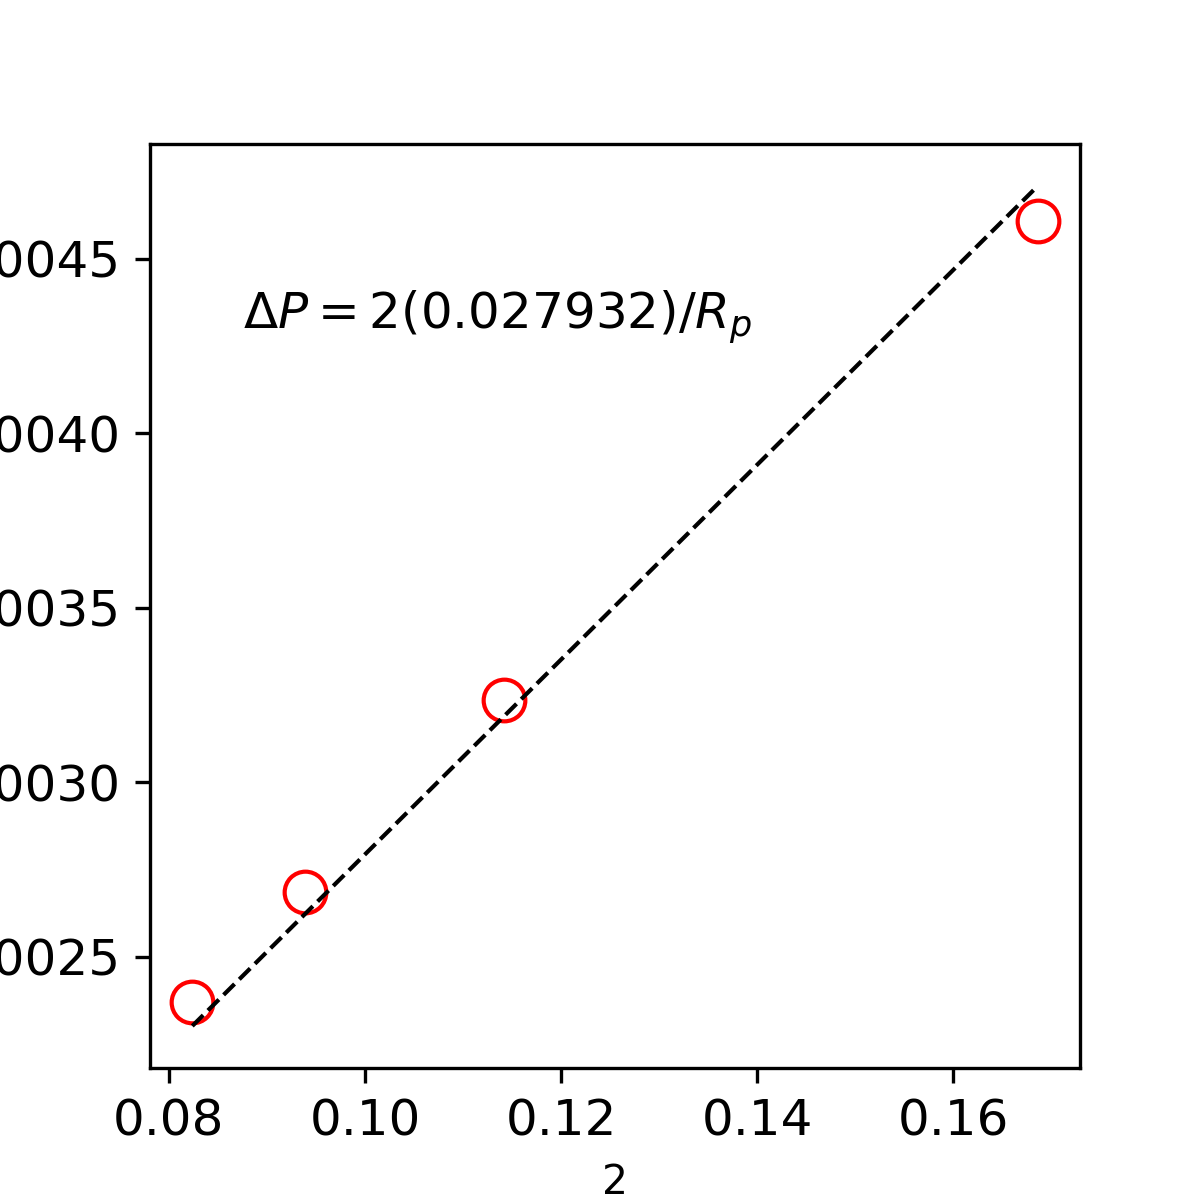
\includegraphics[scale = 0.5]{figures/model_validation/surface_tension.png}
    \caption{Plot of the surface tension of the multicomponent model in this work calculated using the 
    Young-Laplace equation.}
    \label{fig:young_laplace_valid}
\end{figure}

Using the fluid and non-ideal mixing parameters defined in Table \ref{table:model_params}, a single water in oil 
droplet, termed blue in red, was initialized in the center system and run till the droplet radii reached steady state. 
This process was repeated for various droplet diameters, specified between $40$ and $85 \%$ of the system size at $5\%$ 
increments. The system had a box length of $L = 64$ and was run for $50000$ timesteps with periodic boundary conditions 
on all sides. Data was dumped every 10000 timesteps with only the last timestep used to calculate the values shown. Due 
to the diffuse interface present in this method, the density profiles were verified to be at steady state at the end of 
the simulation before further analysis was performed. \cite{frijters_effects_2012} Past work also showed that the 
pressures remained constant after 5 lattice units away from the interface. \cite{frijters_effects_2012} 

The pressure difference was calculated using the difference in scalar pressure between the center of the droplet and 
one of the corners of the box. Two techniques exist to calculate the radius of the droplet. The first directly measures 
the distance between opposite points of the droplet as measured from the density profile at opposite points of the droplet, 
and the second is based upon the total mass and density of the fluid making up the droplet. The second method offers greater 
accuracy by avoiding discretization errors that may exist in the first method, and also allows for the correction of 
particle volume at the interface if the system contained them. First, a local effective mass density 
$\rho^b_{eff} = \rho^{b}_{d} - \rho^{b}_{m}$ is found by calculating the difference in density between the blue 
fluid in the droplet and in the matrix. Next, the droplet mass is calculated as $M_d = \sum_{\mathbf{x}}{\rho_{eff}^{b}}$. 
The radius of the droplet can then be calculated from the mass and density of the droplets as $R_d = \sqrt[3]{\frac{3}{4\pi} 
\frac{M_d}{\rho^b_d - \rho^b_m}}$. To linearize the plot, the $\Delta P$ was plotted against $\frac{2}{R_d}$ with 
$\sigma$ being the slope of the fit.

Figure \ref{fig:young_laplace_valid} shows the results of the fit conducted of the Young-Laplace equation demonstrating 
that under these fluid and mixing parameters, the surface tension is $\sigma = 0.0273$. The fit was performed using 
\texttt{scipy.optimize.curve\_fit} with the fit function defined as $y = mx$. Droplets with starting sizes $2R_d < 70\%$ 
of the initial system size disappeared. This occurred due to the initial condition of each fluid set to not contain the 
other fluid species, meaning once the simulation was initiated diffusion of mass from the droplet to the bulk occurred, 
causing disappearance of the droplet until the thermodynamically optimal composition was reached. From the fit calculated 
in Figure \ref{fig:young_laplace_valid}, the fit is linear as long as the initial droplet size is sufficiently large. 
Alternatively, the composition of the system can be set to near equilibrium in order to allow access to smaller droplet 
sizes.

% \subsection{Contact angle}
% \label{section:model_contact_angle}

% Contact angle plays a role in particle stabilized emulsions by controlling the free energy reduction that the interface 
% has in addition to the imparting of preferential curvature. LB3D allows for modification of the contact angle of a 
% particle through the addition of a shell of blue or red fluid to the surface of the Ladd particle termed as the particle 
% color $(\Delta \rho)$. \cite{jansen_bijels_2011, gunther_lattice_2013} To ensure that the correct settings are used in 
% these simulations, in addition to gaining understanding into how to change parameters if the need arises, the contact 
% angle as a function of the particle color was calculated.

% Experimentally and computationally, the contact angle can be calculated through direct measurement of the angle of a 
% droplet on a substrate. A droplet that preferentially wets a substrate has a lower contact angle relative to that 
% substrate material, physically manifesting as the droplet spreading on the substrate. At a liquid interface, the particle 
% will prefer to be in the particle it wets more. Thus for a spherical particle, the contact angle can be calculated as 
% $\theta_c = \arccos{\frac{h_p - h_i}{R_p}}$ where $h_p - h_i$ defines the distance between the center of the particle 
% after reaching its steady state position and the interface and $R_p$ is the radius of the spherical particle. 
% \cite{gunther_lattice_2013, davies_interface_2014} This has been extended to ellipsoidal particles through assuming 
% that the particle will have its largest cross sectional area flat on the interface and using the radius that is 
% perpendicular to the interface to calculate the contact angle, defined as $\theta_c = \arccos{\frac{h_p - h_i}{R_{\parallel}}}$ 
% and $\theta_c = \arccos{\frac{h_p - h_i}{R_{\perp}}}$ if $\alpha < 1$ and $\alpha \geq 1$ respectively. 

% The simulation was setup in a box of size $32\cdot32\cdot64$ with an interface lying at $z = 32$, and a single particle 
% placed at the center of the box with periodic boundary conditions on all sides. Fluid and non-ideal mixing properties were 
% the same as those listed in table \ref{table:model_params}. The particle was then placed at the center of the simulation 
% box and run for $30000$ timesteps with data read every 500 timesteps. The contact angles shown are results from triplicate 
% runs, and averages of the final 10 data points. 

% \begin{figure}[h]
%     \centering
%     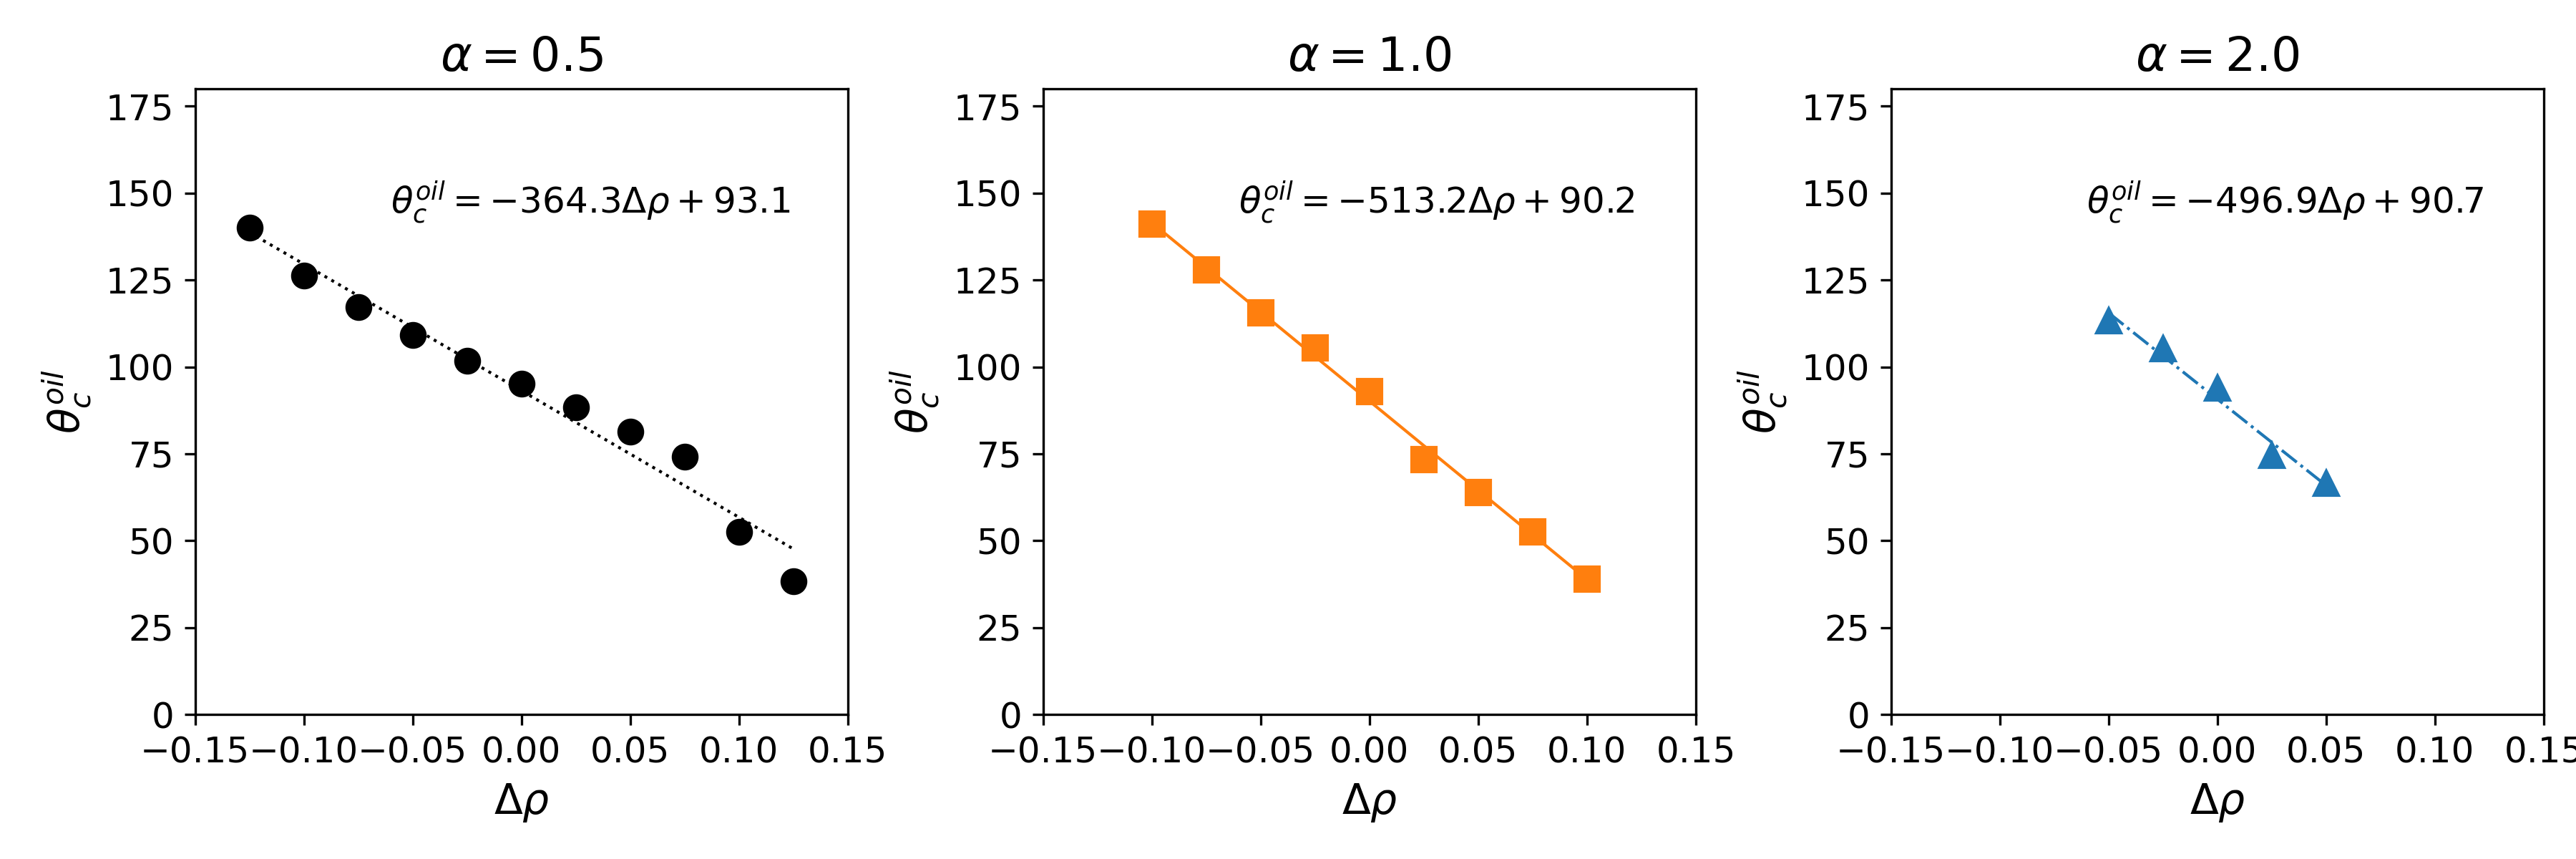
\includegraphics[scale = 0.5]{figures/model_validation/contact_angle_compare.png}
%     \caption{Contact angle with respect to the oil phase, $(\theta_c^{oil})$ of the particles plotted against the 
%     control parameter in LB3D}
%     \label{fig:contact_angle_valid}
% \end{figure}

% Figure \ref{fig:contact_angle_valid} demonstrates the contact angles of the three particle geometries analyzed, 
% confirming that $\Delta \rho = 0$ will result in neutrally wetting particles for all geometries. Oblate and spherical 
% particles have usable particle colors between $-0.10 \leq \Delta \rho \leq 0.10$ while for prolate ellipsoids this 
% value is $-0.05 \leq \Delta \rho \leq 0.05$. The slope of ellipsoidal particles appears to be lower which may arise 
% from a larger interfacial adsorption energy, making it more difficult for surface energy changes to move particles out 
% of the interface. At $\Delta \rho$ values further from 0, it was observed that the prolate particles tended to leave 
% the interface rather than stay at a slightly off center equilibrium position. 